\section{Architecture}

\begin{figure}
  \centering
  \caption{\label{3layers}Robot collaboration software architecture}
  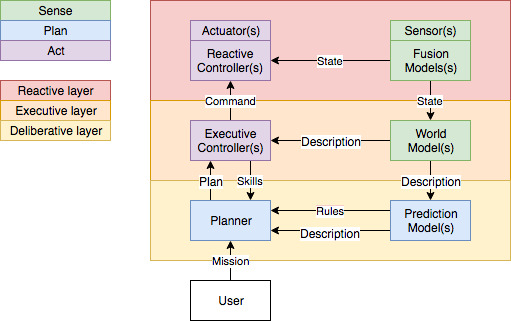
\includegraphics[scale=0.40]{img/3layers}
\end{figure}

The global architecture is a Sense-Plan-Act, but this architecture is not very modular and cannot easily be distributed across several robots.
Also, Sense-Plan-Act is not well suited for the low level control of a robot (especially if the robot is limited in computing power), where Sense-Act is preferred.

The base architecture can be adapted to a 3 layers architecture (Reactive, Executive, Deliberative).
The deliberative layer keebs a Sense-Plan-Act pattern, while the reactive layer will keep the simple and distributed low level control of the robot.

The reactive layer only understand low level, short-termed single commands, while the deliberative layer outputs a plan, consisting of a more or less complex sequence of actions.
The executive layer is here as an adaptation layer between the 2 formers.
It should also be able to express the actions that the planner will be able to use to solve a problem.

\subsection{Discovery}

To collaborate, robots will need the help of the network to discover each other.
We need to discover the robots endpoints (named/addressed data streams) and the type of data exchanged.

The problem solver / planner part will also need to "understand" what kind of actions the robots can do.
The "skills" can be described with a specific language (PDDL, STRIPS, and co), and served by the robots to be downloaded by the planning part.

There is three steps of the discovery : 
First, after the mission is received, the planning system need to discover which actors (robots/IoT devices) can be used.
Then, it need to dicover the skills of each actors.
And finally, and continuously, the environment need to be discovered through prior knoledge, or sensing.

\subsection{Planning}

The planning problem can be splitted in 2 parts (PDDL, STRIPS,...) : 
The domain description, which describe the possible states of the manipulated entities (the environement) and the possible actions (of the robots, in our case).
The problem description, which basically describes the initial state, and the goal state.

In the case of robotics, the initial state is not really known, so that the problem description is meant to change over time, and be splitted in 2 : 

The goal state, which does not changes unless the user decide otherwize.
This is the mission of the robot as described previously.

The "initial state", or the current environment state, which will be updated with discovery and envirnment sensing.
Basically, the planning algorithm will be ran periodically (or on input event) with a different initial state description.

\subsection{Control}

There is 2 types of controllers : 
Reactive controllers, that takes short-termed simple commands, sensors states, and outputs lower leve commands to actuators (or lower level reactive controllers).
Executive controllers, that takes mission plan, environment description, and sends proper commands to one or several reactive controllers.

\subsection{Recursivity}

Considering modularity and different level of description of the environment and tasks, planners can be considered as controllers for higher level planners.
Indeed, if during the global mission plan, an action is to "grab object X", this action can be considered as a mission for a lower level planner, that will schedule each action of the robotic arm to fulfill the mission.

\subsection{bottom-up domain description}

If robots parts can do simple tasks, the parts linked together can do more complex actions that cannot be described in any domain description of the pieces.
There will be a need to automatically compute new possible tasks that can be done by the set of modules, and make it available to the planner.

\subsection{Communication}

\subsubsection{Pub/Sub}

This communication pattern is used when we need the data to be sent to the consumer as fast as possible after it has bee produced.
For example, the data of a sensor that is used in a (realtime) control system.
Also, the commands of an controller that is sent to an actuator (real or virtual).

\subsubsection{Req/Res}

This communication pattern is used when the consumer need a big chunck of data, or data that is not updated often, or when requesting a computation task.
This can be used for example to serve the skills descriptions, where a planned will request only when the robot is discovered.
This can also be used to run some heavy computation on a server if the client is not powerful enough.